\documentclass[11pt,a4paper]{article}

% for Chinese
%\usepackage{fontspec}  % 加這個就可以設定字體
%\usepackage[BoldFont, SlantFont]{xeCJK}  % 讓中英文字體分開設置
%\setCJKmainfont{新細明體}  % 設定中文為系統上的字型,而英文不去更動,使用原TeX\字型

% useful packages
\usepackage{amsfonts}
\usepackage{amssymb}
\usepackage{amsmath}
\usepackage{amsthm}
\usepackage{epsfig}
\usepackage{graphicx}
\usepackage{natbib}
\usepackage{textcomp}
\usepackage{booktabs}
\usepackage{multirow}
\usepackage{url}
\usepackage{color}
\usepackage{fullpage}
\usepackage[capitalize]{cleveref}
\usepackage{mathtools}
\usepackage{enumitem}
\usepackage{authblk}
\usepackage{algorithm}
\usepackage{algpseudocode}
\usepackage{subcaption}
\usepackage{tikz}
\usepackage{pgfplots}
% basic setting
\renewcommand{\baselinestretch}{1.25}
\parskip=5pt
\parindent=20pt
\footnotesep=5mm

% abbreviation
\newtheorem{lem}{Lemma}
\newtheorem{prop}{Proposition}
\newtheorem{thm}{Theorem}
\newtheorem{defn}{Definition}
\newtheorem{cor}{Corollary}
\newtheorem{assp}{Assumption}
\newtheorem{obs}{Observation}
\newenvironment{pf}{\begin{proof}\vspace{-10pt}}{\end{proof}}
% \newtheorem{ques}{Question}
% \newtheorem{rmk}{Remark}
% \newtheorem{note}{Note}
% \newtheorem{eg}{Example}

\newenvironment{enumerateTight}{\begin{enumerate}\vspace{-8pt}}{\end{enumerate}\vspace{-8pt}}
\newenvironment{itemizeTight}{\begin{itemize}\vspace{-8pt}}{\end{itemize}\vspace{-8pt}}
\leftmargini=25pt   % default: 25pt
\leftmarginii=12pt  % default: 22pt
\pgfplotsset{compat=1.17}

\title{Operations Research, Spring 2025 (113-2) \\ Final Project Proposal}

\author{Zi-Yi Jau} % b12705064
\author{Bing-Zhe Wu} % b12705049
\author{Chung-Kai Lin} % b12705052
\author{Zhi-Xin Lin} % b12705013
\author{Nan-Tien Lai} % b12705010
\affil{Department of Information Management, National Taiwan University}



\begin{document}

\maketitle

\section{Introduction}
In modern urban transportation systems, bike-sharing services play a significant role in providing eco-friendly and efficient mobility options. A major challenge in operating such systems is balancing the number of docking stations and available bikes across different locations. Imbalances in supply and demand at stations may lead to service disruptions—specifically, users being unable to rent bikes due to shortages or return them due to full docks. Therefore, optimizing dock allocations based on real usage data is crucial to improving system efficiency and user satisfaction.

\section{Problem description}
This study focuses on optimizing the allocation of docking stations across five hypothetical bike-sharing locations (Stations A–E). We use synthesized data representing bike check-out and return events collected every 15 minutes over a typical day. Analysis of net bike flow at each station reveals imbalances in supply and demand, leading to potential periods of "empty" or "full" stations. The goal is to determine the number of docks to install at each location, within given upper and lower bounds, in a way that minimizes the total service disruption time across all stations.

\section{Mathematical model}
We formulate this as a mixed-integer programming problem. Let:
\begin{itemize}
    \item $s_i$ = number of docks at station $i$ (decision variable)
    \item $d_i^+$ = penalty for excessive returns (station full)
    \item $d_i^-$ = penalty for excessive check-outs (station empty)
    \item $t_i$ = estimated ideal capacity (based on usage)
\end{itemize}

\noindent The objective is:
\[
\text{Minimize} \quad Z = \sum_{i} (d_i^+ + d_i^-)
\]

\noindent Subject to:
\begin{align*}
    s_i^{\min} &\leq s_i \leq s_i^{\max} & \forall i \quad &\text{(station dock limits)} \\
    \sum_i s_i &\leq S_{\text{total}}^{\max} & \quad &\text{(total docks available)} \\
    f(s_i) + d_i^- - d_i^+ &= t_i & \forall i \quad &\text{(demand satisfaction with deviation)} \\
    s_i &\in \mathbb{Z}_{\geq 0}, \quad d_i^+, d_i^- \geq 0 & \quad &\text{(variable domains)}
\end{align*}

\noindent Function $f(s_i)$ can be a proxy based on historical bike flow at station $i$.

\section{Expected results}
The expected output of the model is the optimal number of docks to assign to each station such that total disruption time due to full or empty stations is minimized. This model allows city planners or system operators to evaluate trade-offs between dock capacity and service reliability. By analyzing patterns in bike usage and optimizing dock allocation accordingly, the model is expected to improve user access and reduce the operational challenges associated with imbalances in bike availability. Future enhancements could incorporate dynamic rebalancing and time-of-day adjustments for more adaptive deployment strategies.

\subsection*{Net Flow Visualization}
\begin{center}
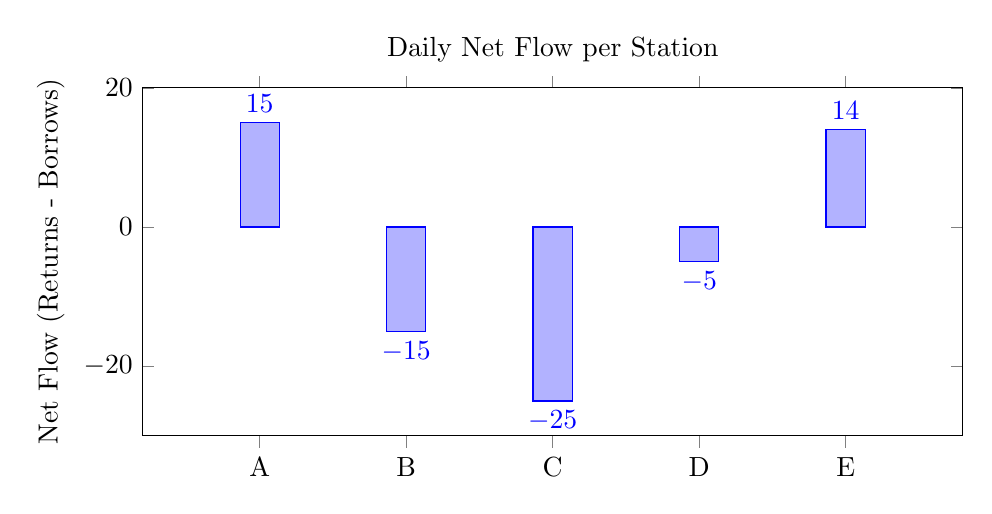
\begin{tikzpicture}
\begin{axis}[
    ybar,
    bar width=.5cm,
    width=12cm,
    height=6cm,
    enlarge x limits=0.2,
    ylabel={Net Flow (Returns - Borrows)},
    symbolic x coords={A, B, C, D, E},
    xtick=data,
    nodes near coords,
    ymin=-30, ymax=20,
    title={Daily Net Flow per Station}
]
\addplot coordinates {(A,15) (B,-15) (C,-25) (D,-5) (E,14)};
\end{axis}
\end{tikzpicture}
\end{center}

\end{document}
